\subsection{Présentation des résultats}

  Finalement, nous avons mis au point, d'une part, une reconnaissance d'image fonctionnelle sur la base de test que nous avions pour travailler, et qui gère les erreurs et, d'autre part, un système automatique permettant de prendre les photos des 6 faces, de les traiter pour initialiser un cube grâce à une fonction intégrable dans le programme Java original. 

  Les résultats obtenus sont ceux des figures~\ref{fig:res1} et ~\ref{fig:res2} qui sont la face 1 et la face 2 d'un cube. 
On observe que la figure~\ref{fig:res1} trouve bien les contours alors que dans la figure~\ref{fig:res2}, la ligne la plus basse de détection de contour (dessinée en noir) n'est pas celle que l'on espérai puisque l'on souhaite détecter les deux lignes séparatrices du milieu pour reconstruire la face du cube. 

  La cause de cette erreur est visible en comparant les courbes rouges qui correspondent aux projections en Y des images. 
On voit que les 2 pics minimaux ne sont pas les mêmes dans ces deux cas. 

  \begin{figure*}[!ht]
    \centering
    %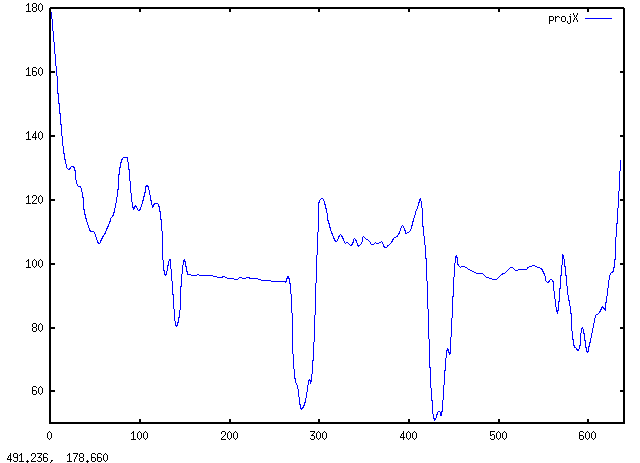
\includegraphics[width=0.4\linewidth]{./Images/projX_1.png}
    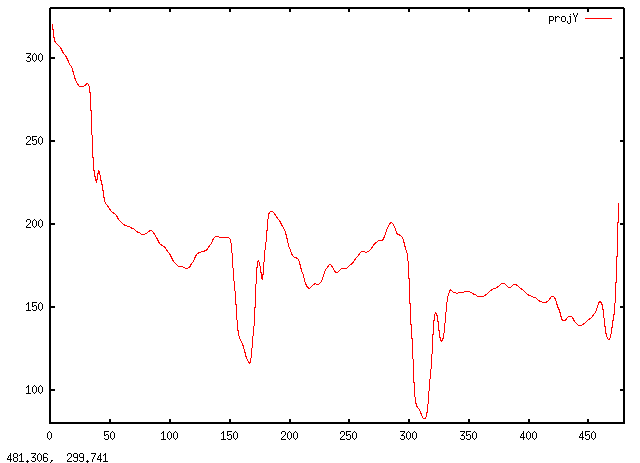
\includegraphics[width=0.4\linewidth]{./Images/projY_1.png}
    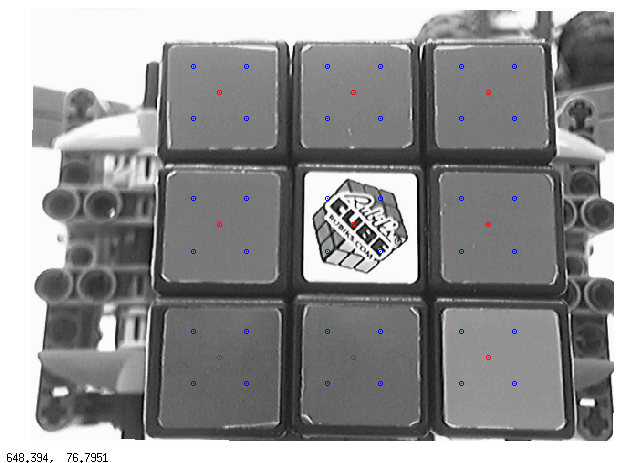
\includegraphics[width=0.4\linewidth]{./Images/face_1.png}
    \caption{Résultat sur une image sans reflet}
    \label{fig:res1}
   \end{figure*}

  \begin{figure*}[!ht]
    \centering
    %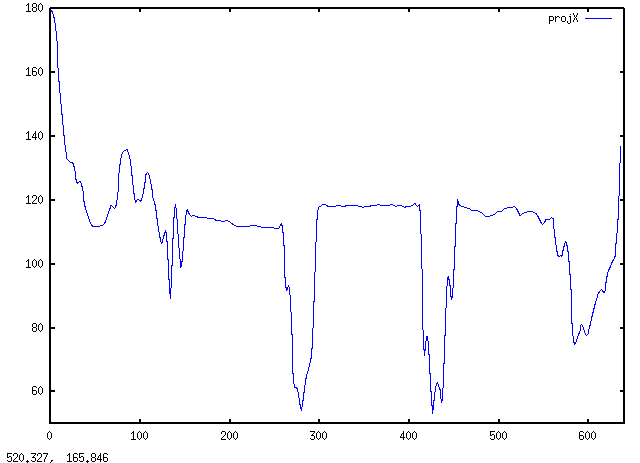
\includegraphics[width=0.4\linewidth]{./Images/projX_2.png}
    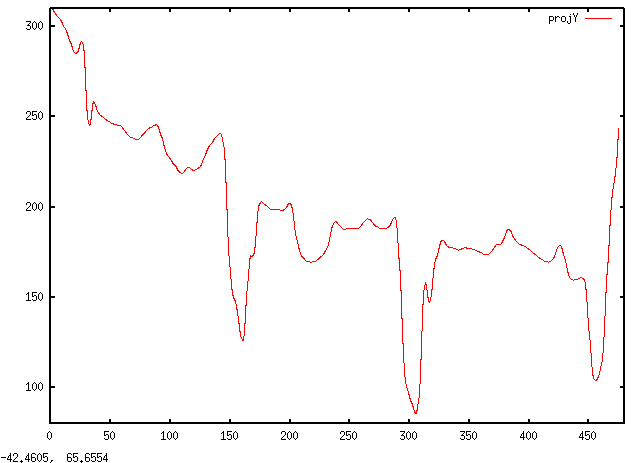
\includegraphics[width=0.4\linewidth]{./Images/projY_2.png}
    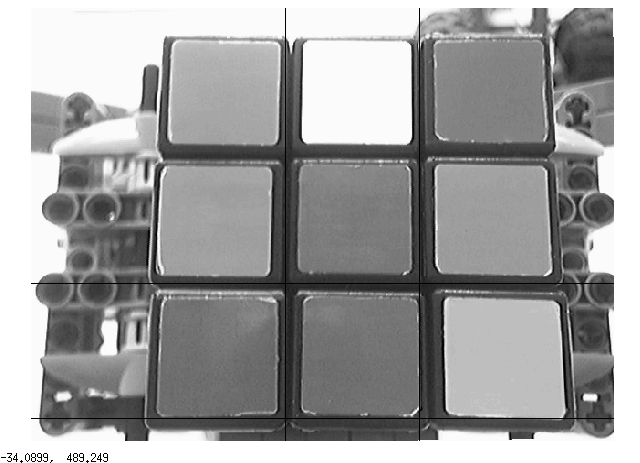
\includegraphics[width=0.4\linewidth]{./Images/face_2.png}
    \caption{Résultat sur une image avec reflet}
    \label{fig:res2}
   \end{figure*}

\textit{Remarque : } Les résultats des figures~\ref{fig:res1} et ~\ref{fig:res2} sont obtenus à partir de la configuration 0 en Annexe~\ref{sec:Aconf}. 

\subsection{Nos impressions}
Lorsque nous avons choisi cette ECAO, nous pensions que le problème posé était simple. Nous devions dans un premier temps mettre en place une série de tests sous matlab dans le but d'intégrer la meilleur solution en java. Cependant au cours de nos expériences, nous nous sommes heurtés à plusieurs problèmes successifs tel que la prise en compte de la couleur de certaines pièces du robot, ou les conditions d'éclairage. 

Notre approche de segmentation a eu pour but de segmenter l'image de la façon suivante : nous détectons 2 lignes noir horizontales et 2 lignes noir verticale pour en déduire la positions de chacune des 9 facettes. Cette approche avait pour but de transformer le problème en un cas particulièrement simple. Ainsi nous pouvions écarter facilement le bruit et éviter l'utilisation d'algorithmes beaucoup plus lourds comme de la reconnaissance de formes. 

Suites à nos résultats, nous remettons partiellement en cause cette approche. En effet, nous n'avons de ce fait pas étudié les résultats d'algorithmes de segmentations classiques qui nous auraient peut-être donnés de meilleurs résultats.

  Cependant, cette ECAO nous a permis de comprendre la complexité des problématiques liées à l'étude d'image. Elle nous a permis de faire appel à plusieurs compétences : vision, data mining, programmation matlab et Java, c'est un projet riche ainsi qu'il faudrait segmenter pour le mener à bien. 
